\begin{figure}[H]
\centering
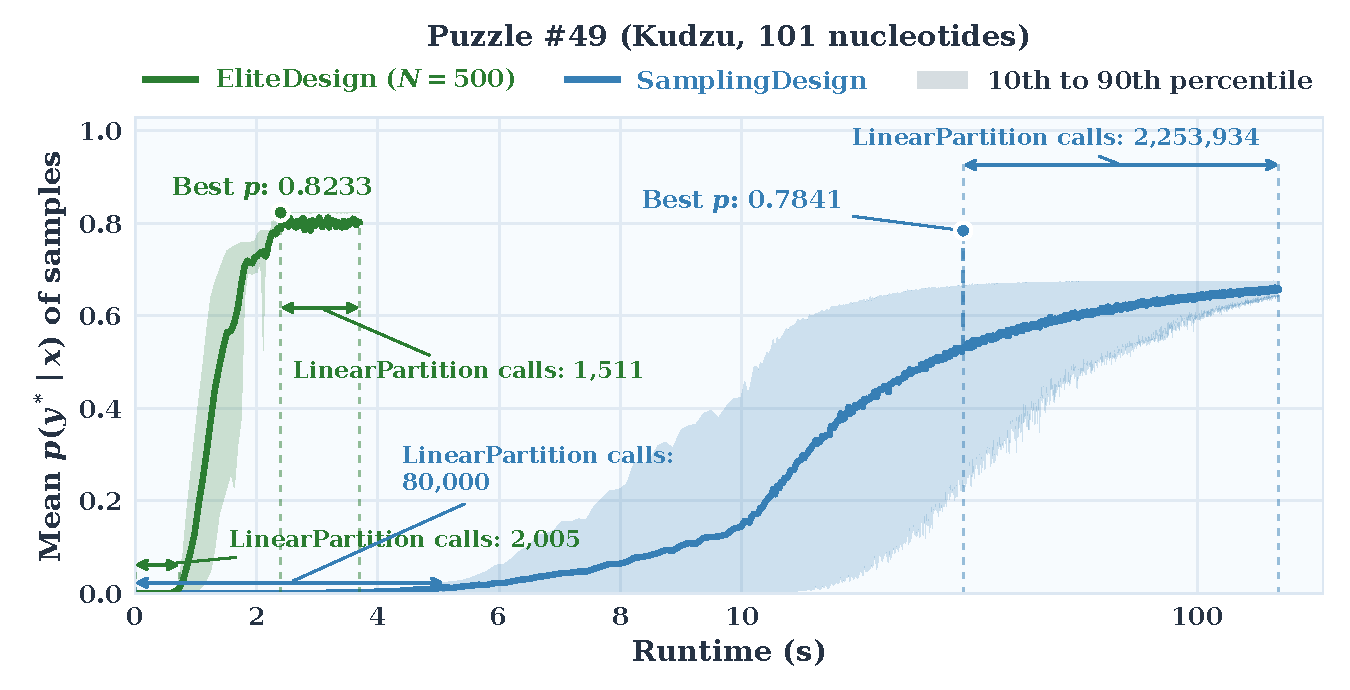
\includegraphics[width=0.92\textwidth]{figures/results/time_p49_prob.pdf}
\caption{Mean Boltzmann probability of the sampled sequences in each round, for EliteDesign ($N=500$) and SamplingDesign with default settings and seed 706, both on 96 cores. Bands show the 10th to 90th percentile, markers show the best probability scored exactly with ViennaRNA, and arrows count how many scoring calls are made to LinearPartition. The runtime axis is linear up to 10 seconds and logarithmic after that.}
\label{fig:trace-p49-prob}
\end{figure}

\begin{figure}[H]
\centering
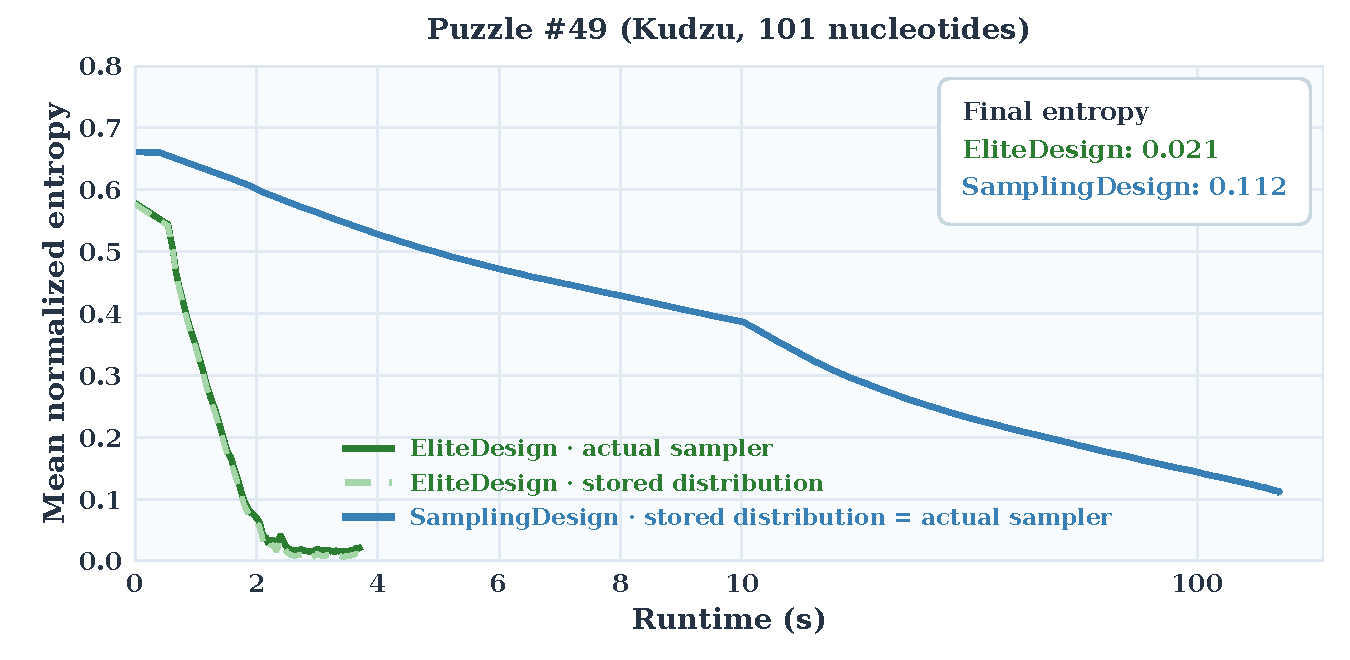
\includegraphics[width=0.92\textwidth]{figures/results/time_p49_entropy.pdf}
\caption{Mean normalized entropy of the sampling distribution in the same runs as Fig.~\ref{fig:trace-p49-prob}. The actual sampler of EliteDesign adds 0.2\% uniform mixing to its stored distribution, while SamplingDesign does not mix. EliteDesign concentrates its distribution in a good region within seconds, so its later samples mostly repeat sequences that were already scored, whereas SamplingDesign keeps a diverse distribution and keeps scoring new sequences.}
\label{fig:trace-p49-entropy}
\end{figure}
